\section{Contribution}

\section{Rail}
\label{rail}
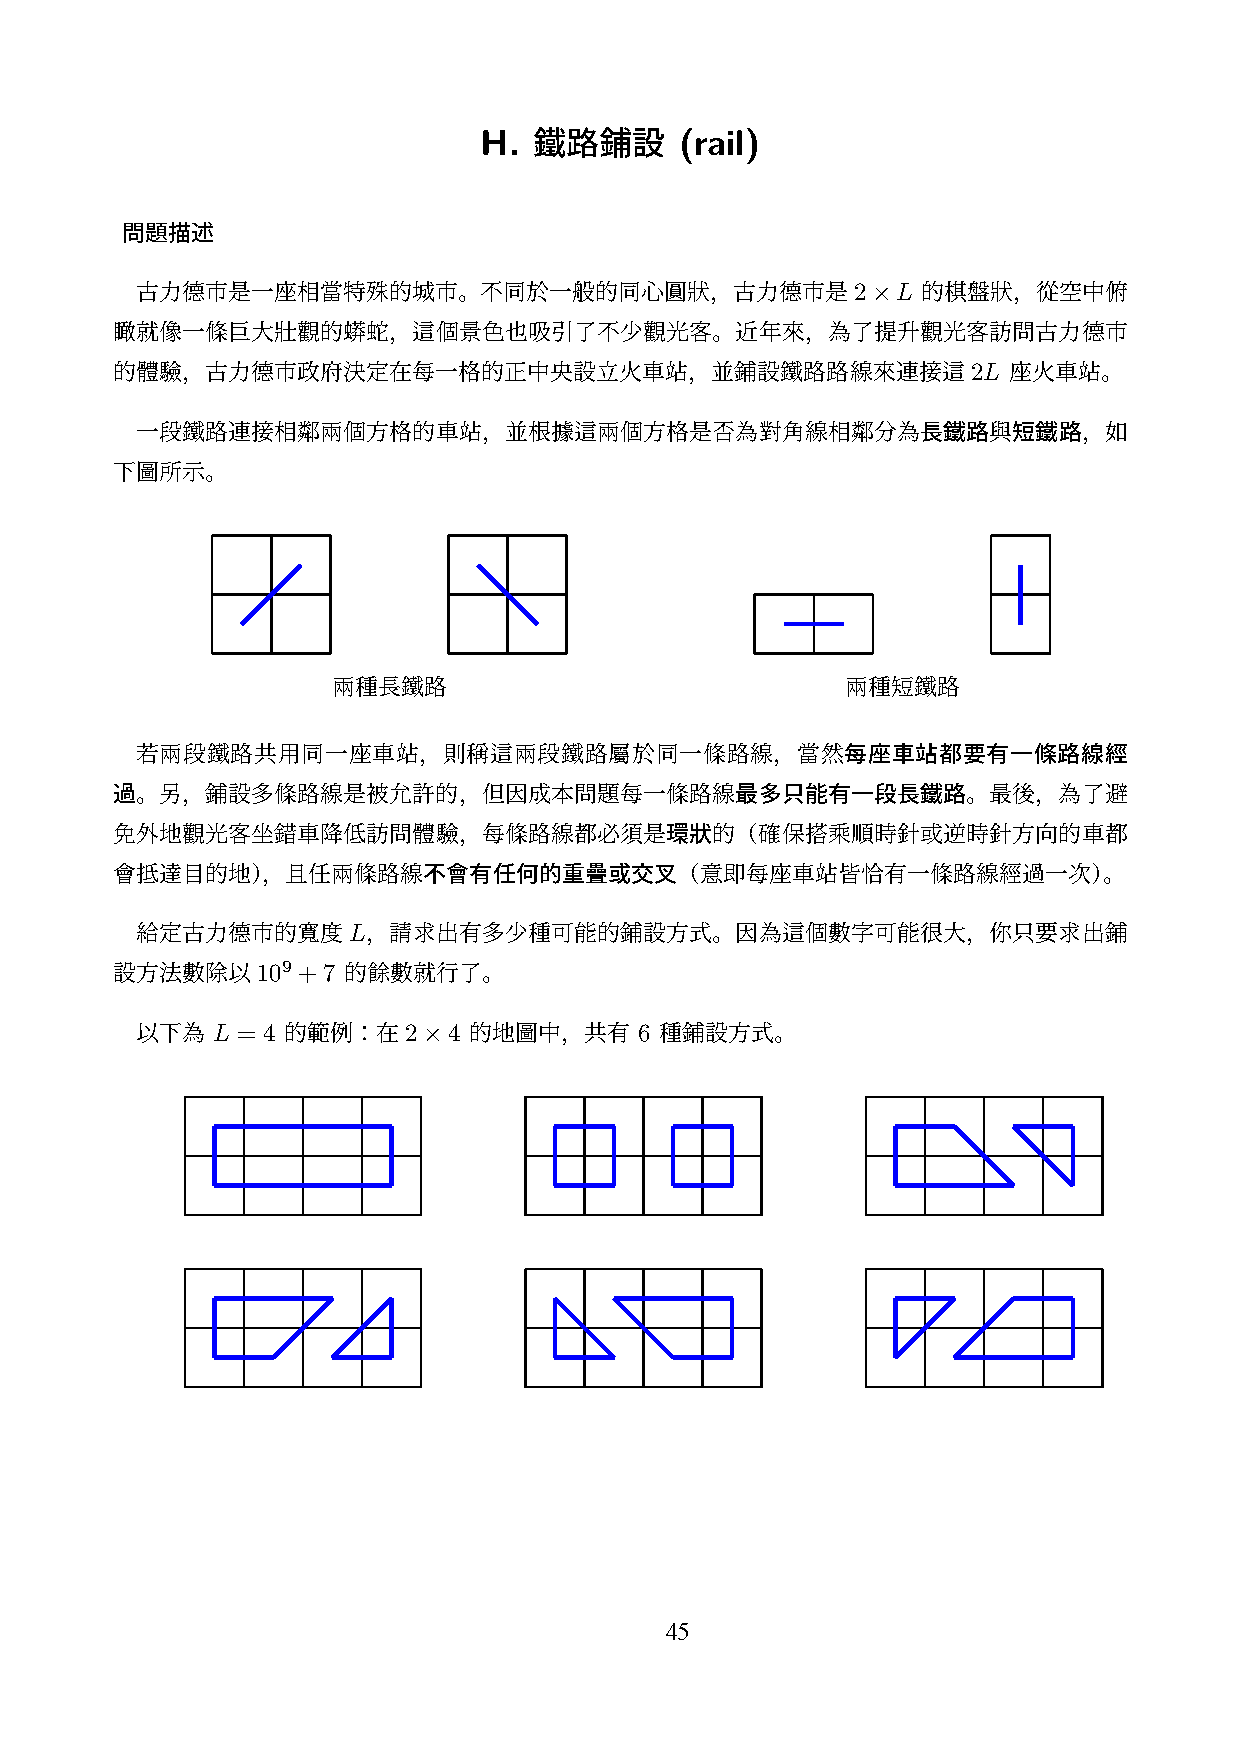
\includepdf[pages=-]{appendices/rail.pdf}

\section{Induction for the Transition Matrix of Rail}
\label{induction for Rail}

\subsection{Induction to recursive formula} 

Divide into 2 cases\\

\begin{enumerate}
    \item[Case 1:] 
        First cycle doesn't have // and cost $k$ blocks. $\rightarrow$ At least need 2 blocks (like Fig \ref{case1}.) and only one method.\\

        $\Rightarrow \sum\limits_{j=0}^{n-2}(1\times D_j)$\\

    \item[Case 2:]
        First cycle have // and cost $k$ blocks. $\rightarrow$ At least need 3 blocks and have multiple methods.\\
        \begin{enumerate}
            \item [1.]
               Have $k-2$ places to choose where // is.\\

            \item [2.]
                Fig \ref{case2-1}. and Fig \ref{case2-2} are two different methods.\\
        \end{enumerate}
        
        $\Rightarrow \sum\limits_{j=0}^{n-3}(2(n-j-2)\times D_j)$
\end{enumerate}

\begin{minipage}{\linewidth}
    \centering
    \begin{minipage}{0.32\linewidth}
        \begin{figure}[H]
            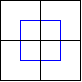
\includegraphics[width=2cm]{picture/case1.png}
            \caption{case 1}
            \label{case1}
        \end{figure}
    \end{minipage}
    % \hspace{0.05\linewidth}
    \begin{minipage}{0.32\linewidth}
        \begin{figure}[H]
            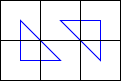
\includegraphics[width=3cm]{picture/case2_1.png}
            \caption{case 2-1}
            \label{case2-1}
        \end{figure}
    \end{minipage}
    % \hspace{0.05\linewidth}
    \begin{minipage}{0.32\linewidth}
        \begin{figure}[H]
            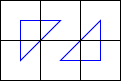
\includegraphics[width=3cm]{picture/case2_2.png}
            \caption{case 2-2}
            \label{case2-2}
        \end{figure}
    \end{minipage}
\end{minipage}

\ \\

Combine both case 1 and case 2, we obtained the recursive formula of $D_i$.

$$D_n = \sum\limits_{j=0}^{n-2}D_j + \sum\limits_{j=0}^{n-3}2(n-j-2)D_j$$

Notice that: For the second sigma, when $j = n-2,\ n-j-2 = n-(n-2)-2 = 0$.\\

Therefore, 

\begin{align*}
D_n &= \sum\limits_{j=0}^{n-2}D_j + \sum\limits_{j=0}^{n-3}2(n-j-2)D_j \\
    &= \sum\limits_{j=0}^{n-2}D_j + \sum\limits_{j=0}^{n-2}2(n-j-2)D_j \\
    &= \sum\limits_{j=0}^{n-2}(2(n-j)-3)D_j 
\end{align*}

\subsection{From recursive formula to transition matrix}

We start with the recursive formula:
\begin{equation}
    D_i = \sum\limits_{j = 0}^{i - 2}(2(i - j) - 3)D_j
\end{equation}

Expanding the summation:
\begin{align*}
    D_i &= \sum\limits_{j = 0}^{i - 2}(2i - 2j - 3)D_j \\
        &= \sum\limits_{j = 0}^{i - 2}(2i - 3)D_j - \sum\limits_{j = 0}^{i - 2}2jD_j \\
        &= (2i - 3)\sum\limits_{j = 0}^{i - 2}D_j - 2\sum\limits_{j = 0}^{i - 2}jD_j
\end{align*}

Using induction, we express $D_i$ and $D_{i - 1}$:
\begin{align}
    D_i &= (2i - 3)\sum\limits_{j = 0}^{i - 2}D_j - 2\sum\limits_{j = 0}^{i - 2}jD_j \label{eq:di} \\
    D_{i - 1} &= (2i - 5)\sum\limits_{j = 0}^{i - 3}D_j - 2\sum\limits_{j = 0}^{i - 3}jD_j \label{eq:di_minus_1}
\end{align}

To simplify further, subtract Equation~\eqref{eq:di_minus_1} from Equation~\eqref{eq:di}:
\begin{align*}
    D_i - D_{i - 1} &= (2i - 3)D_{i - 2} + 2 \sum\limits_{j = 0}^{i - 3}D_j - 2(i - 2)D_{i - 2} \\
                    &= D_{i - 2} + 2\sum\limits_{j = 0}^{i - 3}D_j
\end{align*}

Using induction on the differences, we arrive at:
\begin{align*}
    D_i - D_{i - 1} - D_{i - 2} &= 2\sum\limits_{j = 0}^{i - 3}D_j \\
    D_{i - 1} - D_{i - 2} - D_{i - 3} &= 2\sum\limits_{j = 0}^{i - 4}D_j \\
    D_i - 2D_{i - 1} + D_{i - 3} &= 2D_{i - 3}
\end{align*}

Thus, we obtain the recurrence relation:
\begin{equation}
    D_i = 2D_{i - 1} + D_{i - 3}
\end{equation}

\subsection{Transition Matrix Representation}

We represent this recurrence relation using a transition matrix:
\[
\begin{bmatrix}
    D_i \\
    D_{i - 1} \\
    D_{i - 2}
\end{bmatrix}
=
\begin{bmatrix}
    2 & 0 & 1 \\
    1 & 0 & 0 \\
    0 & 1 & 0
\end{bmatrix}
\begin{bmatrix}
    D_{i - 1} \\
    D_{i - 2} \\
    D_{i - 3}
\end{bmatrix}
\]

The general term can be expressed as:
\[
\begin{bmatrix}
    D_i \\
    D_{i - 1} \\
    D_{i - 2}
\end{bmatrix}
=
\begin{bmatrix}
    2 & 0 & 1 \\
    1 & 0 & 0 \\
    0 & 1 & 0
\end{bmatrix}^{i - 2}
\begin{bmatrix}
    D_2 \\
    D_1 \\
    D_0
\end{bmatrix}
=
\begin{bmatrix}
    2 & 0 & 1 \\
    1 & 0 & 0 \\
    0 & 1 & 0
\end{bmatrix}^{i - 2}
\begin{bmatrix}
    1 \\
    0 \\
    1
\end{bmatrix}
\]

\section{Code for Fibonacci}
\label{Fibonacci Code}
\subsection{Using Recursion}
\lstinputlisting[language=C++]{appendices/fibonacci_recursion.cpp}

\subsection{Using DP}
\lstinputlisting[language=C++]{appendices/fibonacci.cpp}

\subsection{Using Fast Matrix Power}
\lstinputlisting[language=C++]{appendices/fibonacci_bignum_2.cpp}

\section{Code for Rail}
\label{Rail Code}
\subsection{Using Recursion}
\lstinputlisting[language=C++]{appendices/rail_recursion.cpp}
\subsection{Using DP}
\lstinputlisting[language=C++]{appendices/rail.cpp}
\subsection{Using Fast Matrix Power}
\lstinputlisting[language=C++]{appendices/rail_bignum.cpp}